\documentclass{standalone}

\usepackage{tikz}
\usepackage{amssymb}
\usetikzlibrary{calc, positioning}
\begin{document}
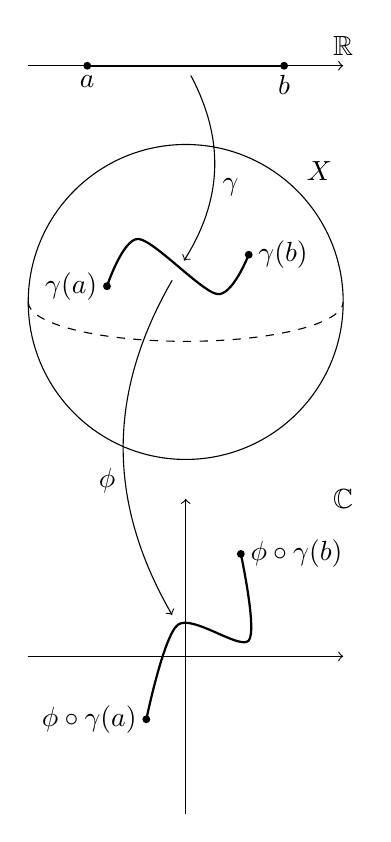
\begin{tikzpicture}
	\draw[->] (-2, 0) to (2,0) node[above]{$ \mathbb{R} $};
	\coordinate (a) at (-1.25,0);
	\coordinate (b) at (1.25,0);
	\fill (a) circle (0.05) node[below]{$ a $};
	\fill (b) circle (0.05) node[below]{$ b $};
	\draw[thick] (a) to (b);
	\node (l) at ($ (a)!0.5!(b) $){};

	\begin{scope}[yshift=-3cm]
		\draw (0,0) circle (2);
		\draw[dashed] (-2,0) arc[start angle=180, end angle=360, x radius=2, y radius=0.5];
		\node[above right] at (45:2) {$ X $};
		\coordinate (a') at (-1,0.2);
		\coordinate (b') at (0.8, 0.6);
		\fill (a') circle (0.05) node[left]{$ \gamma(a) $};
		\fill (b') circle (0.05) node[right]{$ \gamma(b) $};
		\draw[thick] plot[smooth] coordinates {(a') ($ (a') + (0.4,0.6) $) ($ (a') +
					(1.4, -0.1) $) (b')};
		\node (l') at ($ (a')!0.5!(b') $){};
	\end{scope}

	\begin{scope}[yshift=-7.5cm]
		\draw[->] (-2,0) to (2,0);
		\draw[->] (0,-2) to (0,2);
		\node at (2,2){$ \mathbb{C} $};
		\coordinate (a'') at (-0.5,-0.8);
		\coordinate (b'') at (0.7, 1.3);
		\fill (a'') circle (0.05) node[left]{$ \phi \circ \gamma(a) $};
		\fill (b'') circle (0.05) node[right]{$ \phi \circ  \gamma(b) $};
		\draw[thick] plot[smooth] coordinates {(a'') ($ (a'') + (0.4,1.2) $) ($
					(a'') + (1.3, 1) $) (b'')};
		\node (l'') at ($ (a'') + (0.4,1.2) $){};
	\end{scope}


	\draw[->, bend left] (l) to node[right, pos=0.6]{$ \gamma $} (l');
	\draw[->, bend right] (l') to node[left, pos=0.6]{$ \phi $} (l'');

\end{tikzpicture}
\end{document}
